\documentclass[11pt]{article}
%Gummi|065|=)
\title{\textbf{PCA Kernel Notes}}
\author{Lorenzo D'Isidoro}
\date{}

\usepackage{amsmath}
\usepackage{amssymb}
\usepackage{pgfplots}
\usepackage{graphicx}
\usepackage{hyperref}
\graphicspath{ {./images/} }
\newcommand{\R}{\mathbb{R}}

\begin{document}

\maketitle

\section{Overview}
Many machine learning algorithms assume that the training dataset is linearly separable, if not, the PCA kernel can be used to transform it into a smaller linearly separable one.

The aim is to perform a non-linear mapping of \( \) $ n $ dataset features, that cannot be linearly separated, in a new larger space and then apply the standard PCA on it to project the samples into a smaller subspace, which is linearly separable.

N points will be transformed in a new subspace k-dimensional using the map function \( \) $ \Phi $ with \( \) $ (k>>d) $
\begin{equation*}
x_{i} 	\in 	\R^{d} \Rightarrow \Phi(x_{i}):\R^{d} \rightarrow \R^{k} 
\end{equation*} 

\begin{figure}[h]
    \centering
    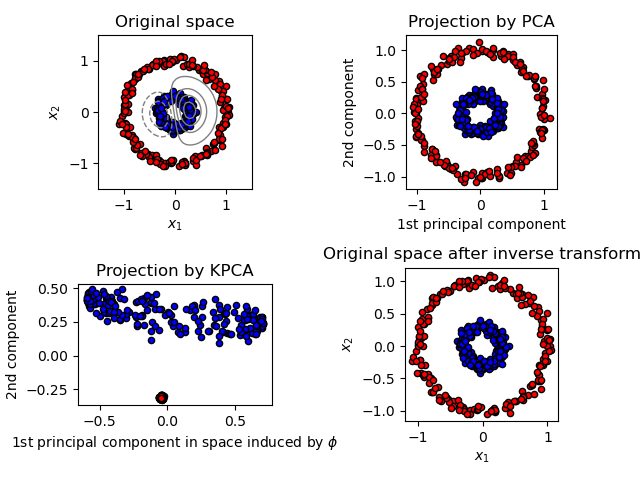
\includegraphics[scale=0.5]{sphx_glr_plot_kernel_pca_001}
    \caption{a plot which show that Kernel PCA is able to find a projection of the data that makes data linearly separable. Source \href{https://scikit-learn.org/stable/auto_examples/decomposition/plot_kernel_pca.html}{scikit-learn.org}}
    \label{fig:mesh1}
\end{figure}




\section{Covariance Matrix}
The elements of the covariance matrix C for the features k and j are
\begin{equation*}
COV(x_j, x_k) = \sigma_{j,k} = \dfrac{1}{n}\sum_{i = 1}^{n} (x^{(i)}_j - \mu_{j})(x^{(i)}_k - \mu_{k})
\end{equation*}

\begin{equation*}
C_{n,d} = 
\begin{pmatrix}
c_{1,1} & c_{1,2} & \cdots & c_{1,n} \\
c_{2,1} & c_{2,2} & \cdots & c_{2,n} \\
\vdots  & \vdots  & \ddots & \vdots  \\
c_{n,1} & c_{n,2} & \cdots & c_{n,d} 
\end{pmatrix}
\end{equation*}

If the features are standardized the avarage \( \) $ \mu_{j} $ and \( \) $ \mu_{k} $ will be 0.

At this point the equation which is used to calculate the covariance matrix is
\begin{equation*}
C = \dfrac{1}{n}\sum_{i = 1}^{n} (x^{(i)})(x^{(i)})^T
\end{equation*}

Apply the map function called \( \) $ \Phi $ to the combination of nonlinear features
\begin{equation*}
C_{map} = \dfrac{1}{n}\sum_{i = 1}^{n} \Phi(x^{(i)})\Phi(x^{(i)})^T = \dfrac{1}{n}\Phi(X)\Phi(X)^T
\end{equation*}

The eigenvalues and eigenvectors can be calculated starting from the following equation
\begin{equation*}
C_{map}v = \lambda v 
\end{equation*}

Where \( \) $ \lambda $ is the vector of the eigenvalues to be used to calculate the eigenvectors and substituting \( \) $ C_{map} $ 
\begin{equation*}
C_{map}v = \lambda v \Rightarrow (\dfrac{1}{n}\sum_{i = 1}^{n} \Phi(x^{(i)})\Phi(x^{(i)})^T)v = \lambda v 
\Rightarrow v = v\dfrac{1}{n\lambda}\sum_{i = 1}^{n} \Phi(x^{(i)})\Phi(x^{(i)})^T
\end{equation*}

\begin{equation*}
\Rightarrow v = \dfrac{1}{n}\sum_{i = 1}^{n} \Phi(x^{(i)})a^{(i)} = \Phi(X)^Ta
\end{equation*}

Then
\begin{equation*}
C_{map}v = \lambda v \Rightarrow (\dfrac{1}{n}\Phi(X)\Phi(X)^T)(\Phi(X)^Ta) = \lambda(\Phi(X)^Ta) 
\end{equation*}

\begin{equation*}
\Rightarrow \dfrac{1}{n}\Phi(X)\Phi(X)^Ta = \lambda a \Rightarrow \dfrac{1}{n}Ka = \lambda a
\end{equation*}

Where K is the kernel matrix \( \) $ K = \Phi(X)\Phi(X)^T $ and the kernel function \( \) $ k(x^{(i)}, x^{(j)}) = \Phi(x^{(j)})\Phi(x^{(i)})^T $.



There are several kernel functions that can be used, \href{https://www.sciencedirect.com/topics/computer-science/kernel-function}{here} can be found a deep understanding about this topic, but in this case will be used the Gaussian form of the kernel function defined as follow

\begin{equation*}
k(x^{(i)}, x^{(j)}) = e^{(-\dfrac{||x^{(i)} - x^{(j)}||^2}{2\sigma})}
\end{equation*}

Where \( \) $ ||x^{(i)} - x^{(j)}|| $ is the squared Euclidean distance between the two feature vectors and \( \) $ \sigma $ is a free parameter, setting the \( \) $ \gamma = \dfrac{1}{2\sigma^2} $ the function can also be written as

\begin{equation*}
k(x^{(i)}, x^{(j)}) = e^{(-\gamma{||x^{(i)} - x^{(j)}||^2})}
\end{equation*}

Since the value of the RBF kernel decreases with distance and ranges between zero and one, when \( \) $ x^{(i)} = x^{(j)}$, source wikipedia.org. The K matrix will be defined as follows

\begin{equation*}
K_{(n,n)} = 
\begin{pmatrix}
k({x^{(1)}, x^{(1)}}) & k({x^{(1)}, x^{(2)}}) & \cdots & k({x^{(1)}, x^{(n)}}) \\
k({x^{(2)}, x^{(1)}}) & k({x^{(2)}, x^{(2)}}) & \cdots & k({x^{(2)}, x^{(n)}}) \\
\vdots  & \vdots  & \ddots & \vdots  \\
k({x^{(n)}, x^{(1)}}) & k({x^{(n)}, x^{(2)}}) & \cdots & k({x^{(n)}, x^{(n)}})
\end{pmatrix}
\end{equation*}

Before selecting the eigenvectors of K the kernel matrix should be centered
\begin{equation*}
K' = K - 1_n K - K1_n + 1_nK1_n
\end{equation*}

Where the matrix \( \) $ 1_n $ is an \( \) $ n x n $ matrix with all values equal to \( \) $ \dfrac{1}{n} $.

\end{document}
